\entete{HTT}{10 Septembre 2010}

\section{Alg\`ebre relationnelle et SQL (10 points)}

Voici une partie de la base de donn\'ees utilis\'ee pour g\'erer les enseignements au CNAM:

\smallskip
\texttt{\textbf{ENSEIGNANT}(id, nom, prenom)}\\
\texttt{\textbf{UE}(id, nom, nb\_credits, id\_ens)}\\
\texttt{\textbf{AUDITEUR}(id, nom, prenom)}\\
\texttt{\textbf{INSCRIPTION}(id\_aud, id\_ue)}\\

(UE: unit\'e d'enseignement, id\_ens: ID enseignant)

%NB : si vous estimez que le sujet ne comporte pas l'ensemble des r\`egles de
%gestion permettant la r\'edaction des requ\^etes, vous pouvez poser des
%hypoth\`eses compl\'ementaires. Dans ce cas, indiquez explicitement ces
%hypoth\`eses sur votre copie.\\

%Pour chacune des questions  \'enonc\'ees ci-dessous, vous donnerez une
%expression alg\'ebrique et/ou une requ\^ete SQL (en fonction de ce qui est
%demand\'e) permettant d'y r\'epondre :


\begin{enumerate}

  \item Pour chaque table identifiez les cl\'es primaires et les cl\'es \'etrang\`eres. (1 point)
  
\begin{correction}
    Table ENSEIGNANT: id: cl\'e primaire\\
    Table UE: id: cl\'e primaire, id\_ens : cl\'e \'etrang\`ere\\
    Table AUDITEUR: id: cl\'e primaire\\
    Table INSCRIPTION : (id\_aud, id\_ue) : clef primaire, id\_aud : clef \'etrang\`ere, id\_ue : clef \'etrang\`ere
\end{correction}

  \item Donnez les commandes SQL permettant de cr\'eer les tables ENSEIGNANT et UE. (1 point)

\begin{correction}
  CREATE TABLE ENSEIGNANT\\
(\\
  id INTEGER NOT NULL,\\
  nom VARCHAR2(15),\\
  prenom VARCHAR2(15),\\
  CONSTRAINT ENSEIGNANT\_pkey PRIMARY KEY (id)\\
) ;\\
CREATE TABLE UE\\
(\\
  id INTEGER NOT NULL,\\
  nom VARCHAR2(15),\\
  nb\_credits INTEGER,\\
  id\_ens INTEGER,\\
  CONSTRAINT UE\_pkey PRIMARY KEY (id),\\
  CONSTRAINT UE\_id\_ens\_fkey FOREIGN KEY (id\_ens)
      REFERENCES ENSEIGNANT (id) \\
) ;
\end{correction}

  \item Donnez les noms des UE qui ont entre 2 cr\'edits et 6 cr\'edits. Alg\`ebre et SQL (1 point)
\begin{correction}
    Alg\`ebre:\\
    $\pi_{nom}(\sigma_{nb\_credits \ge 2 \land nb\_credits \le 6}(UE))$\\
    SQL: \\
    SELECT nom FROM UE\\
    WHERE nb\_credits $>$= 2 AND nb\_credits $<$= 6;
\end{correction}

  \item Donnez le nom de l'enseignant responsable de l'UE de nom 'NFP107'. Alg\`ebre et SQL. (2 points)
\begin{correction}
    Alg\`ebre: Jointure sur l'id de l'enseignant\\
    $\pi_{nom}(\rho_{id \rightarrow id\_ens}(ENSEIGNANT) \Join (\rho_{nom \rightarrow nom\_ue}(\sigma_{nom='NFP107'}(UE)))$\\
    SQL:\\
    SELECT e.nom FROM ENSEIGNANT e, UE u\\
    WHERE e.id = u.id\_ens AND u.nom = 'NFP107';\\
\end{correction}

  \item Donnez le nom de chaque auditeur avec la somme de ses cr\'edits. SQL seulement. (1 point)
\begin{correction}
  SELECT a.nom, sum(nb\_credits)\\
  FROM AUDITEUR a, UE u, INSCRIPTION i\\
  WHERE a.id = i.id\_aud and u.id=id\_ue\\
  GROUP BY a.id, a.nom
\end{correction}
  
  \item Donnez les noms des auditeurs inscrits à une UE de 4 cr\'edits enseign\'ee par Laurent Blanc? Alg\`ebre et SQL. (3points)
\begin{correction}
  Alg\`ebre:\\
	$A = \rho_{id \rightarrow id\_ens (\sigma_{nom='Blanc' \land prenom='Laurent'}(ENSEIGNANT))} $ (liste des IDs des enseignants appel\'es Laurent Blanc)\\
    $B = \rho_{id \rightarrow id\_ue}(\sigma_{nb\_credits=4}(UE))$ (Liste des UE de 4 cr\'edits)\\
    $Resultat = \pi_{nom}((\rho_{id \rightarrow id\_aud}(AUDITEUR)) \Join ( INSCRIPTION \Join (A \Join B)))$\\ 
   SQL:\\
    SELECT a.nom FROM AUDITEUR a, UE u, INSCRIPTION i, ENSEIGNANT e\\
    WHERE i.id\_aud=a.id AND id\_ue=u.id AND
          u.id\_ens=e.id AND nb\_credits=4 AND
          e.prenom='Laurent' AND e.nom='Blanc';
\end{correction}

  
  \item Donnez les noms et les pr\'enoms des auditeurs inscrits \`a tous les UE. Alg\`ebre seulement. (1 point)
\begin{correction}
  $\pi_{nom, prenom}(\rho_{id \rightarrow id\_aud}(AUDITEUR) \Join(INSCRIPTION \div \rho_{id \rightarrow id\_ue}(\pi_{id}(UE))))$
\end{correction}
  
\end{enumerate}
 
% \end{enumerate}
 
\section{Index et optimisation  (6 points)}

\begin{enumerate}
  \item On souhaite cr\'eer un index B+Tree d'ordre 2 sur les cours. Donner les diff\'erentes \'etapes d'\'eclatement de l'arbre apr\`es l'insertion successive des valeurs suivantes (2 points) :
  \begin{center}
  NFP107, NFE204, NFE106, NFA011, NFP121, NFE205, NFA001, NFE114, NFE111, NFA112, NFE112
  \end{center}
\begin{correction}
  \begin{figure}[ht]
  \centering
 % 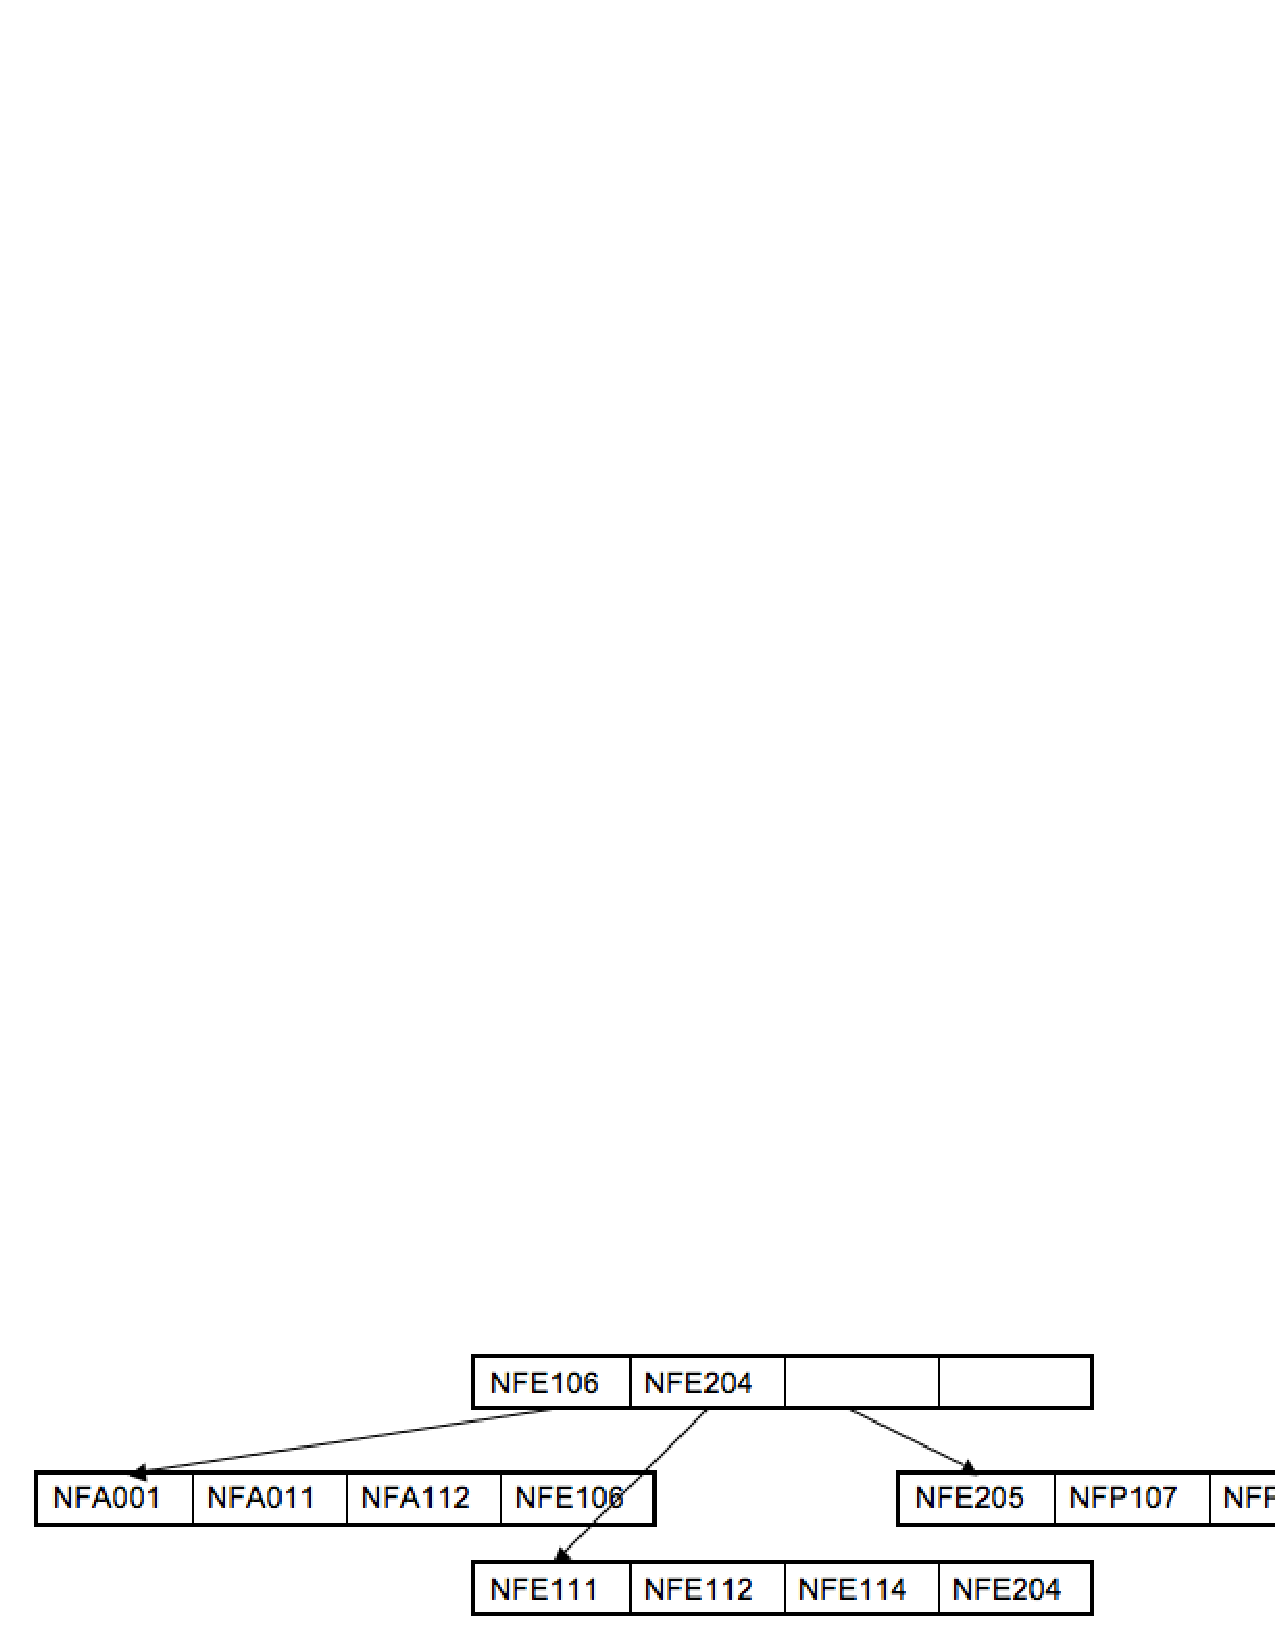
\includegraphics[width=12cm]{Fig/2011-09_btree}
  \end{figure}
\end{correction}


 	\item Soit le plan EXPLAIN suivant. Expliquer ce qu'il calcule et proposer une
 	requ\^ete SQL qui produirait ce plan d'ex\'ecution (2 points) : ~
    \begin{verbatim}
    0 SELECT STATEMENT
    1   NESTED LOOP JOIN
    2*    TABLE ACCESS BY INDEX ROWID  ENSEIGNANT
    3*      INDEX RANGE SCAN           IDX_ENSEIGNANT_NOM
    4*    TABLE ACCESS BY INDEX ROWID  UE
    5*      INDEX RANGE SCAN           IDX_UE_ID_ENS

    (2) ENSEIGNANT.prenom = 'Michel'
    (3) ENSEIGNANT.nom = 'Crucianu'
    (4) UE.nb_credits = 6
    (5) UE.id_ens = ENSEIGNANT.id
    
    \end{verbatim}
    (Les lignes ci-dessus correspondent aux pr\'edicats associ\'es \`a l'op\'erateur)
\begin{correction}\begin{lstlisting}[language=SQL]
     Select u.nom
     From ENSEIGNANT e, UE u
     Where e.id=u.id_ens AND
           e.prenom = 'Michel' and e.nom = 'Crucianu' and
           u.nb_credits = 6 ;
     \end{lstlisting}
\end{correction}
 
  \item Soit la requ\^ete suivante:
      \begin{lstlisting}[language=SQL]
     Select id_ue
     From AUDITEUR a, INSCRIPTION i
     Where a.id = i.id_aud AND
           nom = 'Dupont';
     \end{lstlisting}
     Donner un plan d'ex\'ecution (arborescente ou EXPLAIN) produit par l'optimiseur 
     en argumentant votre r\'eponse, sachant qu'il existe:
     \begin{itemize}
       \item Un index sur INSCRIPTION.\underline{id\_UE}
       \item La table AUDITEUR compte 1000 pages 
       \item La table INSCRIPTION compte 1000 pages
     \end{itemize}
  
  \item  Indiquez   les pr\'edicats associ\'es \`a chaque
  op\'erateur en dessous du plan précédent (1 point).
\begin{correction}
     Comme les deux tables ont m\^eme taille et qu'il n'y a pas d'index sur l'attribut de jointure, on utilisera un tri-fusion (l'index est sur id\_ue\ldots).
    \begin{verbatim}
    0 SELECT STATEMENT
    1*  MERGE JOIN
    2     SORT JOIN
    3*      TABLE ACCESS FULL          AUDITEUR
    2     SORT JOIN
    3       TABLE ACCESS FULL          INSCRIPTION
 
    (1) AUDITEUR.id = INSCRIPTION.id_ue
    (3) AUDITEUR.nom = 'Dupont'
    \end{verbatim}
\end{correction}

\end{enumerate}	

\section{Concurrence (4 points)}

Soit l'ex\'ecution concurrente suivante de trois transactions dans un SGBD.

$$
H: r_1[x] r_2[x] r_3[y] w_1[x] w_1[z] r_3[z] C_1 w_2[z] C_2 w_3[y] C_3
$$

\begin{enumerate}
   \item (1 pt) V\'erifiez si H est s\'erialisable, en trouvant les conflits et en
    construisant son graphe de s\'erialisation.

\begin{correction}
 Conflits :
      sur x: r2[x] - w1[x]
      sur y: rien
      sur z: w1[z] - r3[z], w1[z] - w2[z], r3[z] - w2[z]

      Graphe de s\'erialisation: T1  T3   T1

 Il y a deux cycles, donc H n'est pas s\'erialisable.
\end{correction}     

   \item (1 pt) Existe-t-il une ``lecture sale'' (lecture d'une donn\'ee modif\'ee
   par une autre transaction mais pas encore valid\'ee). Pourquoi faut-il \'eviter
   ce type de lecture (expliquer les effets possibles)\,?

\begin{correction}
Oui, $T_3$ lit $z$ apr\`es modification par $T_1$. Danger potentiel\,: $T_1$
choisit d'annuler, et $T_3$ se retrouve avec une valeur incorrecte pour $z$.
\end{correction}

     \item (2 pts) Quelle est l'ex\'ecution obtenue par verrouillage \`a deux phases
   \`a partir de $H$? On consid\`ere que le relachement des verrous d'une
   transaction se fait au Commit et qu'\`a ce moment on ex\'ecute en priorit\'e les op\'erations bloqu\'ees
      en attente de verrou, dans l'ordre de leur blocage.
\begin{correction}
       r1[x] s'ex\'ecute\\
      r2[x] s'ex\'ecute aussi, car on peut partager le verrou de lecture\\
      r3[y] s'ex\'ecute\\
      w1[x] est bloqu\'ee par r2[x]\\
      w1[z] est bloqu\'ee, car T1 est bloqu\'ee\\
      r3[z] s'ex\'ecute\\
      c1 est bloqu\'ee, car T1 est bloqu\'ee\\
      w2[z] est bloqu\'ee par r3[z]\\
      c2 est bloqu\'ee, car T2 est bloqu\'ee\\
      w3[y] s'ex\'ecute\\
      c3 s'ex\'ecute et relache les verrous de T3 \`a w2[z] peut s'ex\'ecuter et c2\\
      aussi, qui relache les verrous de T2 \`a w1[x], w1[z] et c1 s'ex\'ecutent\\

      R\'esultat: r1[x] r2[x] r3[y] r3[z] w3[y] c3 w2[z] c2 w1[x] w1[z] c1
\end{correction}
\end{enumerate}